\documentclass{article}%
\usepackage[T1]{fontenc}%
\usepackage[utf8]{inputenc}%
\usepackage{lmodern}%
\usepackage{textcomp}%
\usepackage{lastpage}%
\usepackage{authblk}%
\usepackage{graphicx}%
%
\title{Frequent methylation and oncogenic role of microRNA{-}34b/c in small{-}cell lung cancer}%
\author{Erika Shea}%
\affil{Department of Pediatrics and Molecular and Cellular Oncology, The University of Texas M. D. Anderson Cancer Center, Houston, TX, USA}%
\date{01{-}01{-}2013}%
%
\begin{document}%
\normalsize%
\maketitle%
\section{Abstract}%
\label{sec:Abstract}%
A four{-}year NIH clinical trial using ferumoxytol compound (M{-}CHW1) to activate tumorigenesis in triple negative breast cancer cells has shown promise in promising prognostic data, according to interim results from a phase III study of the compound published in the American Journal of Clinical Pharmacology (IJCP) on Dec. 14.\newline%
The clinical trial enrolled the longest randomized{-}type triple negative breast cancer patient populations, a population of patients who have been diagnosed with or are candidates for triple negative breast cancer but are not fully chemo{-} or radiation{-}resistant. Patients in the trial were already on two forms of hormone therapy to treat estrogen receptor{-}positive and hormone receptor{-}negative patients with metastatic triple negative breast cancer.\newline%
Inflammation and insulin response was the primary laboratory biomarkers for tumorigenesis and improved response to ferumoxytol treatment, according to the interim results from the phase III clinical trial, which looked at 34 evaluable triple negative patients. Patients treated with ferumoxytol had no significant increase in the prevalence of white blood cell markers.\newline%
The positive interim results were independent of the CHM{-}CHW2, H2, and Y markers. The encouraging interim findings from the study supplement findings from a 16{-}month phase II clinical trial in which at least 30 percent of patients showed evidence of tumorigenesis in at least one of the three tumor subtypes  evidence that suggests tumorigenesis occurs after tumor suppression, the interim findings of the study support the rationale for using ferumoxytol to stimulate tumorigenesis in triple negative patients.\newline%
Blocking tumorigenesis might reduce the burden of chemotherapy at the tumor site, according to co{-}investigator Omkar Katche, M.D., M.Sc., associate professor of oncology and member of the Stein Center for Clinical Trials at the University of Michigan and chair of the review committee. "This investigator{-}directed study has previously demonstrated that thrombocytopenia and a lack of platelet weight decreases tumorigenesis in triple negative patients, which leads to a relatively high overall survival benefit. The new results from this exciting phase III trial suggest we may be able to expand the use of ferumoxytol to include patients with other types of tumorigenesis."\newline%
Research on transplant rejection and whooping cough recently concluded that ferumoxytol offers a promising anti{-}recurrence of auto{-}immune disease, according to Karamti S. Rohr, M.D., study co{-}investigator and clinical nurse specialist at SRCP, S.L. Bruckmann Hospital in Paris.\newline%
"This new interim result from the phase III study is strong evidence of a potential therapy for one of the most{-}wanted questions for the treatment of breast cancer  whooping cough," Rohr said. "We hope the interim data can eventually be used to direct investigators to consider ferumoxytol for use in breast cancer."\newline%
Rohr added that more preclinical data are needed, but he believes that the overall clinical results from the study are promising.\newline%
Scientists from the University of Michigan, the University of Pennsylvania, the University of Illinois, the University of Montreal, the University of Georgia, the University of Warwick, Oregon Health and Science University, the University of Utah, the University of Buffalo, and the University of Texas, Austin, were co{-}investigators on the interim study.

%
\subsection{Image Analysis}%
\label{subsec:ImageAnalysis}%


\begin{figure}[h!]%
\centering%
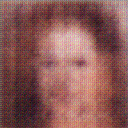
\includegraphics[width=150px]{500_fake_images/samples_5_487.png}%
\caption{A Man In A Suit And Tie In A Room}%
\end{figure}

%
\end{document}